%!TEX root = ../thesis.tex
The original basis for this thesis was born from a fascination of things that moves, adapts and changes.
The the bringing of ``life'' to the objects that surrounds us, letting them transform to our needs, both in function and form. 
Like Theo Jansen's that gives life to new species of animals with his amazing Strandbeests \cite{strandbeestJansen}. 
Made mostly from yellow plastic tube and fabric sails, these skeletons traverses the beaches of the Netherlands, living off the wind, adapting to the turnings of the elements.

The fascination of giving life to inanimate objects is not entirely new.
A famous example of this is the Vaucanson Duck, an automata created by the French inventor and artist Jacques Vaucanson in 1739 \citep{riskin2003defecating}.
The mechanical duck, which supposedly contained over a thousand parts, could both flap its wings and appeared to have the ability to eat, digest, and defecate grains.
These two examples, each impressive in their own right, points to the powerful expressiveness that actuation can give objects, as we have a tendency to relate things that move to living entities.  

\begin{figure}[h]
	\centering
	\begin{minipage}{.45\textwidth}
		\centering
		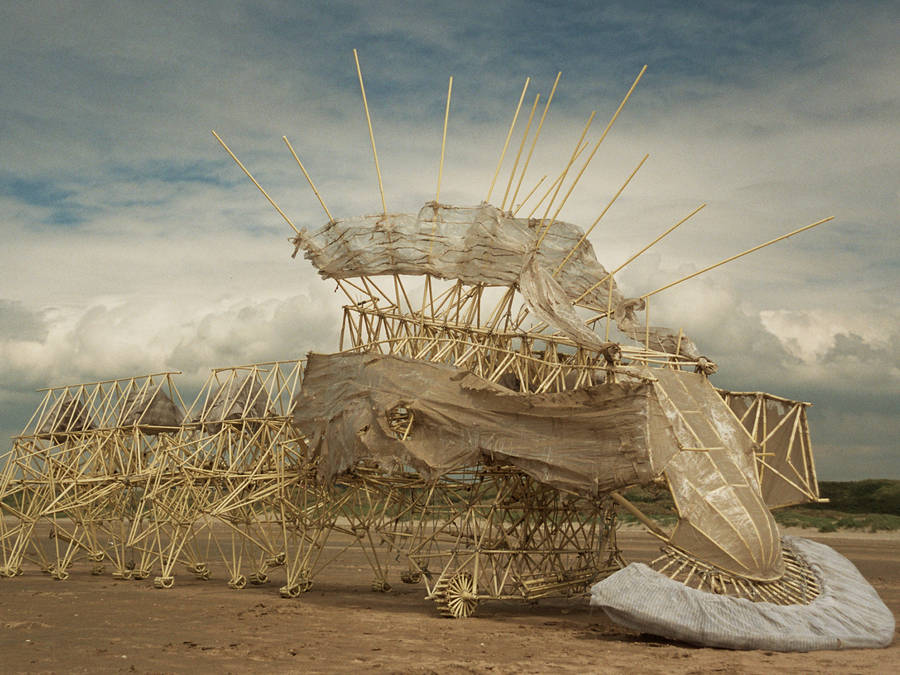
\includegraphics[width=0.9\linewidth]{figures/strandbeest}
		 \captionof{figure}{One of Jansen's amazing Strandbeests, \cite{strandbeestJansen}}
		\label{strandbeest}
	\end{minipage}%
	\hspace{0.1cm}
	\begin{minipage}{.45\textwidth}
		\centering
		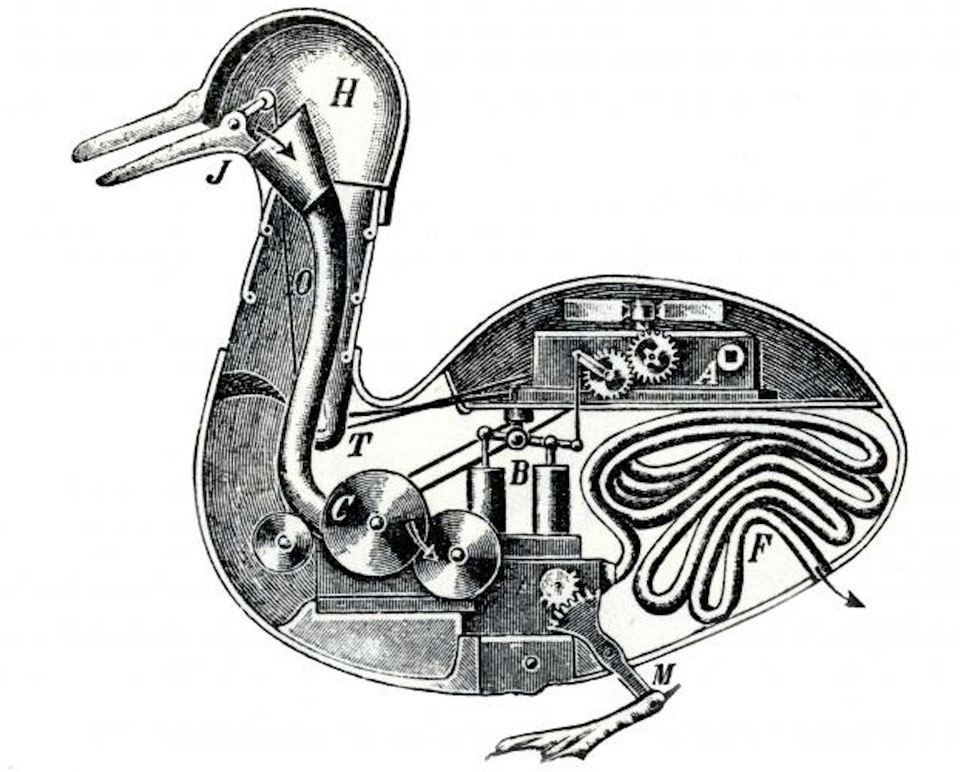
\includegraphics[width=0.9\linewidth]{figures/vaucanson_duck}
		\captionof{figure}{A nineteenth-century inventor's imagined version, depicting the inner workings of the Vaucanson Duck \citep{riskin2003defecating}}
		\label{vaucanson_duck}
	\end{minipage}	
\end{figure}

Noter:
\begin{verbatim}
Hvad er status nu og her og hvad er mulighederne
- ``men, der er faktisk et rum som ikke er udforsket'' - det tidslige, situerede

Computerfokus vs brugerfokus
- Contextual interfaces vs Ad hoc interfaces
- Hvordan kan man give brugeren kontrollen tilbage (i modsaetning til CA)
- Refererende perspektiv - Participatory design - demokratisere - empower the user
- Eksempelvis: end-user-programming
- Tilgangen peger paa et design rum

Hjemmet
- Hvad er et hjem
- Vi fokuserer paa hjemme - en valgt begraensning/omraade med potentiale
- S. Brand og struktur
- Hvad hjemmet betyder for dem der bor der

DIY og infrastruktur
- Balance mellem producent og bruger
- Traditionelle crafts (fra Coelho)

Digital vs fysisk
- Materialitet (shapechange, digital bits)


Afslutte med en aabning til projektet - hvordan vi med udgangspunkt i ovenstaaende har bevaeget os videre, hvad vil vi udforske.
\end{verbatim}